\chapter{Introducción al aprendizaje por refuerzo}

\section{Aprendizaje por refuerzo y agentes}
El \textbf{aprendizaje por refuerzo} (\textit{reinforcement learning}, RL) es una rama del aprendizaje automático que se centra en cómo los agentes deben tomar decisiones para maximizar alguna noción de recompensa acumulada a lo largo del tiempo. A diferencia de otros enfoques de aprendizaje, el RL permite a los agentes aprender a través de la interacción directa con su entorno, ajustando sus estrategias en función de las consecuencias de sus acciones.

Los \textbf{agentes} se definen como programas de software capaces de operar de manera autónoma, percibiendo su entorno mediante sensores y actuando sobre él mediante actuadores.

Un agente inteligente se define por las siguientes propiedades fundamentales:

\begin{itemize}
    \item \textbf{Autonomía:} opera sin intervención humana directa, controlando sus propias acciones y estado interno.
    \item \textbf{Percepción y acción:} recoge información del entorno mediante sensores y actúa sobre él mediante actuadores.
    \item \textbf{Objetivo o función de recompensa:} tiene un criterio claro de éxito que guía su comportamiento.
    \item \textbf{Adaptabilidad:} modifica su comportamiento a partir de experiencias previas o nueva información.
    \item \textbf{Persistencia:} actúa de forma continua a lo largo del tiempo.
\end{itemize}

\subsection*{Tipos de agentes inteligentes}

Existen varios tipos de agentes según su complejidad y modelo de decisión:

\begin{itemize}
    \item \textbf{Agente reactivo simple:} responde directamente a las percepciones actuales sin tener en cuenta el historial. \\
    \textit{Ejemplo:} un termostato.
    
    \item \textbf{Agente basado en modelo:} mantiene una representación interna del entorno para tomar decisiones más informadas. \\
    \textit{Ejemplo:} un robot de limpieza que recuerda obstáculos.

    \item \textbf{Agente basado en objetivos:} actúa para alcanzar objetivos específicos, no solo para reaccionar. \\
    \textit{Ejemplo:} un agente de búsqueda en un videojuego.

    \item \textbf{Agente basado en utilidad:} toma decisiones optimizando una función de utilidad que puede incorporar múltiples objetivos y prioridades. \\
    \textit{Ejemplo:} un sistema de recomendación personalizado.
\end{itemize}

\section{Procesos de decisión de Markov (MDP)}

Un MDP es un marco matemático utilizado para modelar la toma de decisiones en situaciones donde los resultados son en parte aleatorios y en parte bajo el control de un agente.

Son esenciales en el RL porque proporcionan la estructura matemática para modelar y resolver problemas en los que un agente debe aprender a tomar decisiones óptimas a través de la interacción con su entorno.

Se compone de:

\begin{itemize}
    \item \textbf{Estados (S):} representan todas las posibles situaciones en las que puede encontrarse el agente.
    
    \item \textbf{Acciones (A):} conjunto de todas las acciones posibles que el agente puede realizar en cada estado.
    
    \item \textbf{Transiciones (T):} definen la probabilidad de pasar de un estado a otro al realizar una acción específica. \\
    Formalmente, $T(s, a, s') = P(s' \mid s, a)$, donde:
    \begin{itemize}
        \item $s$ es el estado actual,
        \item $a$ es la acción tomada,
        \item $s'$ es el estado siguiente.
    \end{itemize}
    
    \item \textbf{Recompensas (R):} cuantifican la ganancia inmediata tras transitar de un estado a otro por medio de una acción. \\
    Formalmente, $R(s, a, s')$ es la recompensa recibida al pasar de $s$ a $s'$ mediante la acción $a$.
    
    \item \textbf{Política ($\pi$):} es la estrategia que sigue el agente para decidir qué acción tomar en cada estado. \\
    Puede representarse como $\pi(a \mid s)$, que indica la probabilidad de tomar la acción $a$ en el estado $s$.
\end{itemize}

\subsection*{Política óptima y política estacionaria}

\begin{itemize}
    \item \textbf{Política óptima ($\pi^*$):} es la estrategia que maximiza el rendimiento esperado a largo plazo desde cualquier estado inicial. Representa la mejor política que un agente puede seguir para obtener el mayor beneficio esperado.

    \item \textbf{Política estacionaria:} es aquella en la que la decisión del agente depende únicamente del estado actual y no del instante de tiempo. \\
    Esto implica que si el agente se encuentra varias veces en un mismo estado, ejecutará siempre la misma acción, independientemente del momento. \\
    Las políticas estacionarias simplifican el análisis y la implementación en algoritmos de aprendizaje por refuerzo.
\end{itemize}

\subsection*{Utilidad}

La utilidad es una medida del valor o satisfacción que un agente obtiene a partir de una secuencia de decisiones o resultados. Se utiliza para evaluar y comparar distintas políticas.

\begin{itemize}
    \item \textbf{Utilidad aditiva:} el valor total de una trayectoria se calcula como la suma directa de las recompensas recibidas en cada paso:
    \[
    U = \sum_{t=0}^{T} R_t
    \]

    \item \textbf{Utilidad ponderada:} cada recompensa se multiplica por un factor de ponderación $\omega_t$, permitiendo priorizar ciertas decisiones:
    \[
    U = \sum_{t=0}^{T} \omega_t \cdot R_t
    \]

    \item \textbf{Utilidad descontada:} las recompensas futuras se reducen en valor mediante un factor de descuento $\gamma \in [0,1)$. Es ampliamente utilizada en aprendizaje por refuerzo:
    \[
    U = \sum_{t=0}^{\infty} \gamma^t \cdot R_t
    \]
    Este enfoque permite equilibrar entre recompensas inmediatas y futuras.
\end{itemize}

La \textbf{utilidad total} en un proceso de decisión secuencial se define como la suma de las recompensas futuras descontadas. Este concepto es clave en el aprendizaje por refuerzo, ya que permite al agente equilibrar la \textit{explotación} de recompensas inmediatas con la \textit{exploración} de recompensas futuras.

Formalmente, si $R_t$ representa la recompensa obtenida en el instante $t$, y $\gamma \in [0,1)$ es el factor de descuento, entonces la utilidad total $U$ se expresa como:

\[
U = \sum_{t=0}^{\infty} \gamma^t \cdot R_t
\]

Este modelo de utilidad es utilizado en algoritmos fundamentales del aprendizaje por refuerzo, como el \textbf{Q-learning} y los algoritmos basados en \textbf{política de valor}.


\section{Ecuaciones de Bellman}
Las \textbf{ecuaciones de Bellman} proporcionan una formulación matemática que descompone un problema de decisión secuencial en subproblemas más simples. Son fundamentales tanto en optimización dinámica como en aprendizaje por refuerzo, especialmente en entornos modelados como procesos de decisión de Markov (MDP).

\subsubsection*{Conceptos clave}

\begin{itemize}
    \item \textbf{Estado ($s$):} representa la situación actual del agente.
    \item \textbf{Acción ($a$):} decisión que el agente puede tomar desde un estado determinado.
    \item \textbf{Recompensa ($r$):} beneficio inmediato obtenido al tomar una acción en un estado.
    \item \textbf{Política ($\pi$):} estrategia que define qué acción tomar en cada estado.
    \item \textbf{Valor ($V$):} utilidad esperada total que se puede obtener al partir de un estado $s$ y seguir una política determinada.
\end{itemize}

Las ecuaciones de Bellman permiten calcular recursivamente el valor de cada estado, considerando todas las recompensas futuras esperadas, lo que resulta clave para definir políticas óptimas.

La \textbf{ecuación de Bellman} para una política $\pi$ se expresa como:

\[
V^{\pi}(s) = \mathbb{E} \left[ r_t + \gamma V^{\pi}(s_{t+1}) \mid s_t = s, \pi \right]
\]

Donde:
\begin{itemize}
    \item $V^{\pi}(s)$ es el valor del estado $s$ siguiendo la política $\pi$.
    \item $r_t$ es la recompensa inmediata al tomar la acción $a$ en el estado $s$.
    \item $\gamma$ es el factor de descuento ($0 \leq \gamma < 1$).
    \item $s_{t+1}$ es el estado siguiente.
    \item La esperanza $\mathbb{E}$ se toma sobre todas las acciones y estados posibles, dado que se sigue la política $\pi$.
\end{itemize}

Las ecuaciones de Bellman permiten descomponer un problema de decisión secuencial en subproblemas más simples. Son fundamentales en algoritmos como \textit{value iteration}, \textit{policy iteration} y \textit{Q-learning}, ya que ayudan a encontrar la política óptima que maximiza la recompensa esperada a largo plazo.







\section{Aplicaciones}

\textbf{1. Conducción autónoma}

El aprendizaje por refuerzo profundo se aplica en:
\begin{itemize}
    \item Optimización de trayectorias y planificación del movimiento.
    \item Estacionamiento automático, cambio de carril con Q-learning y adelantamientos seguros.
    \item Ejemplo: \textit{AWS DeepRacer}, un coche autónomo que aprende a conducir mediante RL en una pista física.
\end{itemize}

\textbf{2. Automatización industrial}

\begin{itemize}
    \item Robots RL realizan tareas peligrosas para humanos.
    \item Ejemplo destacado: DeepMind optimiza el enfriamiento de centros de datos de Google, reduciendo un 40\% del consumo energético mediante decisiones basadas en RL.
\end{itemize}

\textbf{3. Comercio y finanzas}

\begin{itemize}
    \item RL decide cuándo comprar, vender o mantener activos.
    \item Mejora la coherencia frente a decisiones humanas.
    \item Ejemplo: plataforma financiera de IBM que calcula recompensas según ganancias o pérdidas.
\end{itemize}

\textbf{4. Procesamiento del lenguaje natural (PLN)}

\begin{itemize}
    \item Aplicaciones: resumen automático, respuesta a preguntas, traducción y generación de diálogos.
    \item Ejemplo: investigadores de Stanford y Microsoft Research utilizan RL profundo para generar conversaciones coherentes e informativas mediante agentes virtuales.
\end{itemize}

\textbf{5. Atención sanitaria}

\begin{itemize}
    \item Se aplican políticas óptimas de tratamiento sin modelos matemáticos previos.
    \item Usos en regímenes de tratamiento dinámico (DTR), diagnóstico automatizado y optimización de resultados a largo plazo.
    \item RL considera efectos retardados de los tratamientos.
\end{itemize}

\textbf{6. Ingeniería y producción a gran escala}

\begin{itemize}
    \item Ejemplo: plataforma \textit{Horizon} de Facebook, utilizada para:
    \begin{itemize}
        \item Personalizar sugerencias y notificaciones.
        \item Optimizar calidad de vídeo según el estado del buffer y condiciones de red.
    \end{itemize}
\end{itemize}

\textbf{7. Recomendación de noticias}

\begin{itemize}
    \item RL se adapta a cambios en preferencias del usuario.
    \item Se definen recompensas en función de clics, compartidos, actualidad, contexto, etc.
    \item Considera tanto características de las noticias como del lector y el entorno.
\end{itemize}



\begin{figure}[ht]
    \centering
    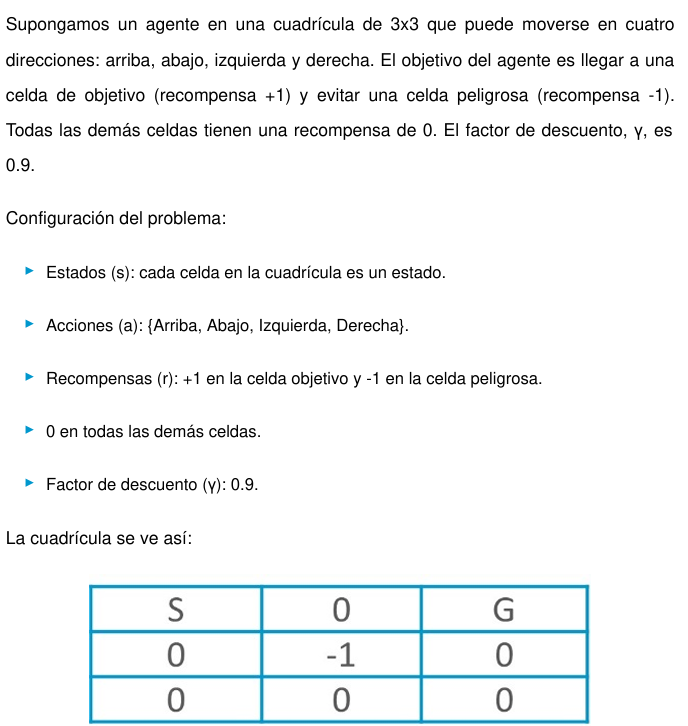
\includegraphics[width=0.55\linewidth]{imagenes/bellman1.png}

\end{figure}

\begin{figure}[ht]
    \centering
    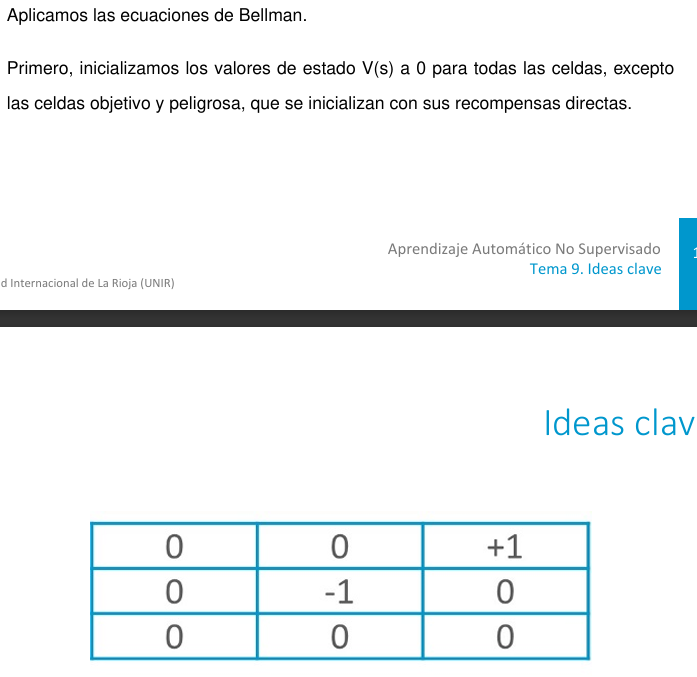
\includegraphics[width=0.55\linewidth]{imagenes/bellman2.png}

\end{figure}

\begin{figure}[ht]
    \centering
    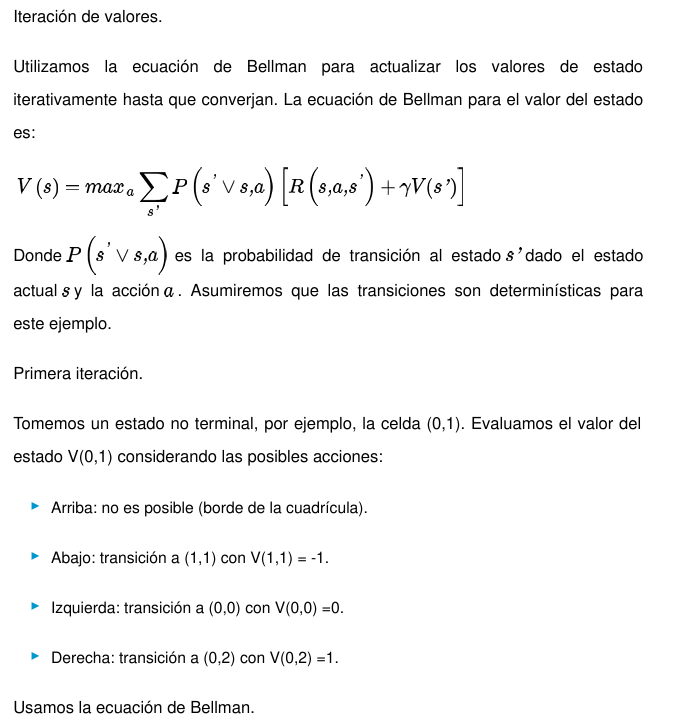
\includegraphics[width=0.55\linewidth]{imagenes/bellman3.png}

\end{figure}

\begin{figure}[ht]
    \centering
    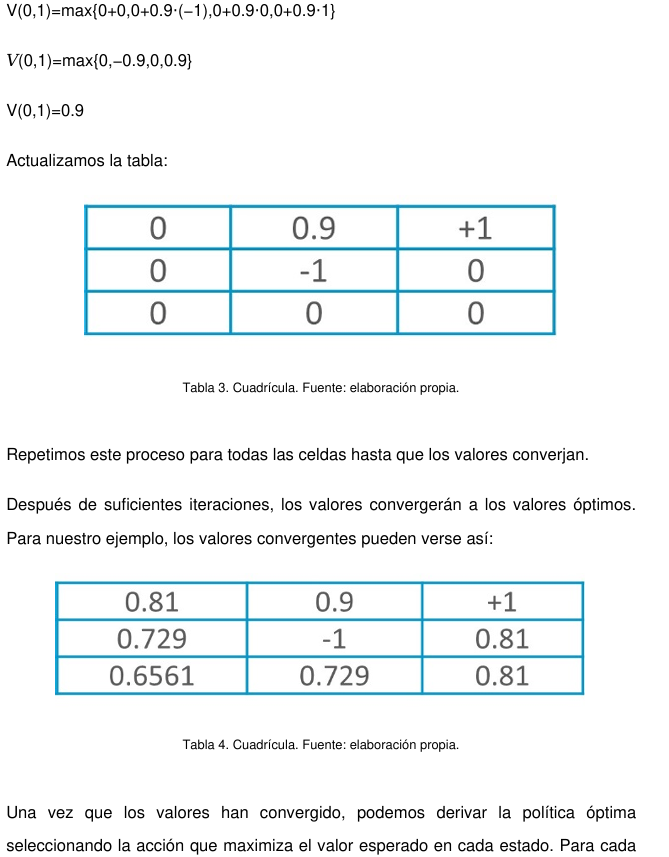
\includegraphics[width=0.55\linewidth]{imagenes/bellman4.png}

\end{figure}